%\documentclass[article,submit,moreauthors,pdftex,10pt,a4paper]{elsarticle}
\documentclass[preprint,12pt]{elsarticle}

%\usepackage{natbib}
\usepackage{graphicx}
\usepackage{amssymb,amsmath,amsthm,amsfonts}
\usepackage[section]{placeins}
\usepackage{hyperref}
%\usepackage{lineno}
%\usepackage{multirow}
\usepackage{float}
\usepackage{adjustbox}
\usepackage{pdflscape}
\hypersetup{
	colorlinks=true,
	linkcolor=blue,
	filecolor=magenta,      
	urlcolor=cyan,
}

%\linenumbers

%%%%%%%%%%%%%%%%%%%%%%%
%% Elsevier bibliography styles
%%%%%%%%%%%%%%%%%%%%%%%
%% To change the style, put a % in front of the second line of the current style and
%% remove the % from the second line of the style you would like to use.
%%%%%%%%%%%%%%%%%%%%%%%

%% Numbered
%\bibliographystyle{model1-num-names}

%% Numbered without titles
%\bibliographystyle{model1a-num-names}

%% Harvard
\bibliographystyle{model2-names.bst}\biboptions{authoryear}

%% Vancouver numbered
%\usepackage{numcompress}\bibliographystyle{model3-num-names}

%% Vancouver name/year
%\usepackage{numcompress}\bibliographystyle{model4-names}\biboptions{authoryear}

%% APA style
%\bibliographystyle{model5-names}\biboptions{authoryear}

%% AMA style
%\usepackage{numcompress}\bibliographystyle{model6-num-names}

%% `Elsevier LaTeX' style
%\bibliographystyle{elsarticle-num}
%\bibliographystyle{elsarticle-harv}
%%%%%%%%%%%%%%%%%%%%%%%

%\journal{Agricultural Economics}
\makeatletter
\def\ps@pprintTitle{%
	\let\@oddhead\@empty
	\let\@evenhead\@empty
	\def\@oddfoot{\hfill\today}%
	\let\@evenfoot\@oddfoot}
\makeatother


%-----------------------------------------------------------------
\begin{document}

\begin{frontmatter}

\title{Payments for Ecosystem Services and Food Security in the Drylands: Experimental Evidence from a REDD+ Intervention in Burkina-Faso}

%% Group authors per affiliation:
%\author{Guigonan Serge Adjognon\corref{mycorrespondingauthor}\fnref{myfootnote1}}
%\fntext[myfootnote1]{Economist, Development Impact Evaluation (DIME), The World Bank Group (WBG).}
%\author{Daan van Soest\fnref{myfootnote2}}
%\fntext[myfootnote2]{Professor, Department of Economics, Tilburg University, Netherlands}
%\author{Jonas Guthoff\fnref{myfootnote3}}
%\fntext[myfootnote3]{Consultant, Development Impact Evaluation (DIME), The World Bank Group (WBG)}

%\address{World Bank Group, 1818 H Street, NW, Washington, D.C. 20433}

\author[label1]{Guigonan Serge Adjognon\corref{mycorrespondingauthor}}
\author[label2]{Daan van Soest}
\author[label1]{Jonas Guthoff}
\address[label1]{Development Impact Evaluation; The World Bank, Washington D.C., USA}
\address[label2]{Professor, Department of Economics, Tilburg University, Netherlands}

\cortext[mycorrespondingauthor]{Correspondence: gadjognon@worldbank.org, Tel.: +1-202-473-0222}



\begin{abstract}
Can environmental cash transfer programs improve the welfare of participants? We answer this question using data from a large scale afforestation intervention implemented as part of the Burkina Faso Forest Investment Plan (FIP). The intervention enrolled selected farmers living around targeted forests in tree planting activities, and offered them monetary payments based on the number of trees still alive, after verification, almost a year later. Leveraging a random allocation of individual participation status amongst community members, to identify treatment effects, we find that participation in the intervention improved significantly food security during the pre-harvest period when these farmers are most vulnerable to food insufficiency. This is important as it suggests the existence of opportunities for policy makers to leverage synergies across environmental and social protection goals in order to achieve maximum returns to development investments.


\end{abstract}

\begin{keyword}
\texttt Burkina Faso \sep PES \sep Food Security \sep REDD+
\end{keyword}

\end{frontmatter}



\newpage 
\section{Introduction}
Climate change and food insecurity are coexisting issues at the heart of the Sustainable Development Goals (SDGs). By 2030, the international development community aims to eradicate poverty (SDG1), end hunger (SDG2), and combat climate change and its impacts (SDG13), amongst other goals. With just slightly more than a decade remaining and with dwindling resources policy makers need, more than ever, to create synergies between sectors of development, to maximize the reach of their investments. This study seeks to inform such possibilities, by imbedding a Randomized Controlled Trial in the Burkina Faso Forest Investment Program (FIP), to evaluate whether a policy intervention geared toward climate mitigation targets could also deliver welfare outcomes such as food security.
\\

Policies to conserve forests and to restore habitats make up an important part of the portfolio of activities governments implement to combat climate change. Since the 2015 Paris Agreement, when countries from 196 countries committed to Nationally Determined Contribution (NDC) towards fighting climate change, there has been mounting popularity for global and country-led initiatives such as the REDD+, the Bonn Challenge, the African Forest Landscape Restoration Initiative (AFR100), etc., all of which put some strong emphasis on restoring degraded landscapes while fighting poverty in developing countries. While there is broad agreement these efforts are necessary, there remains discussions as to which policy tools can effectively deliver the desired outcomes. 
At the heart of this debate are the so-called Payments for Ecosystem Services (PES). PES are formally defined as “…voluntary transactions between ecosystem services users and ecosystem services providers that are conditional on agreed rules of natural resource management for generating off site services” (Wunder, 2015). While they vary substantially in their implementation, PES often entail offering monetary incentives to individuals or communities conditional on the provision of well-defined environmental services. Proponents of the tool argue that, in addition to offering strong incentives for environmental conservation, PES have the potential to also deliver socio economic and welfare outcomes, making it an ideal tool for tackling both the climate change and poverty-related issues. In theory, as poor community members get to be involved in PES schemes, the monetary transfers received might serve a social protection role like Conditional Cash Transfer Programs (CCTs) (Alix-Garcia et al., 2018; Pagiola et al., 2005). 
However, there is no rigorous evidence from the available literature suggesting so. Recent reviews of the literature on PES have concluded to mixed results on environmental effectiveness and a critical dearth of counterfactual-based empirical studies of PES effectiveness on socio-economic and welfare outcomes (Borner et al. 2017; Samii et al. 2014). 
\\

To help fill this gap, we partnered with the government of Burkina-Faso and imbedded an impact evaluation into a pilot REDD+ project called Participatory Forest Management (PGFC/REDD+ from its French acronym). The project was part of the Burkina-Faso Forest Investment Plan (FIP) with financing from the Climate Investment Fund (CIF), and Co-supervision by the World Bank and the African Development Bank (AfDB).  The main objective of the project is to improve carbon sequestration capacity of gazetted forests while reducing poverty in rural areas. As part of this program, the communities living the targeted forests were invited every hear to participate in afforestation campaigns targeting selected gazetted forests in the country. These campaigns involved tree planting activities in well-defined areas of the forests in exchange for immediate cash. After tree planting, groups of individuals were enrolled into PES contracts, whereby they would receive additional payments based on trees survival rate. \\

The impact evaluation imbedded in the project was designed to answer the following main research question: What is the impact of participating in the Burkina Faso FIP PES schemes on participants’ food security?  With widespread food insecurity exacerbated by climate change affecting the reliability of rains during the only one rainy season enjoyed by farmers per year, this question is of great relevance for the government.  
\par
Our identification strategy relies on randomly assigning representatives of 630 households from settlements neighboring 11 gazetted forests to a treatment and control group. The participants are almost exclusively farmers who are dependent on the forest for household inputs like fuel wood. Those assigned to the treatment group were grouped into teams of five and were informed that they had the opportunity to earn money, as a group, when maintaining and keeping alive newly planted trees on a given reforestation parcels. They were given PES contracts that stated that their group would receive about \$0.70 for every tree that was still alive almost a year later, and that each of them would receive 20\% of the total amount received. 
\par 
We collected baseline data from both the treatment and control groups before the PES contracts were signed, using a structured multi-module household survey instrument.  Four months after the payments were made, we collected endline data using a similar survey instrument.
\\

The results from the data analysis indicate that participants in the PES scheme experienced significantly less food insecurity than non-participants (See figure below). Our primary measure of food insecurity is the Household Food Insecurity Access Scale - HFIAS (Coates et al., 2007). However, the results are robust to alternative measures including the Household Hunger Scale - HHS (Ballard et al., 2011). This suggests that participation in the PES schemes shielded farmers against food insecurity at a time where they were most prone to it. The payments coincided with the pre-harvest period where very few farmers still have stocks from the previous harvest. \\

The rest of this paper is organized as follows. 
 



%\newpage 
%\section{Theoretical/Conceptual Framework}



\newpage 
\section{Program Description and Experimental Design}

Forest conservation has become central in international climate policies. This is demonstrated by the rising popularity of REDD+\footnote{Reducing Emissions from Deforestation and Forests Degradation} initiatives in many developing countries, since the 2015 Paris agreement. As the urgency of climate action is acknowledged worldwide, it is also widely accepted that forests represent a cost effective source of carbon sequestration regulating climate, while providing economic, environmental, and socio-cultural benefits \citet{canadell2008managing}. In recent years, an increasing development budget has been pledged to forest conservation interventions (World Bank, 2016).  \\

In this spirit, the Government of Burkina-Faso has been implementing a Forest Investment Plan (FIP) with joint technical assistance from the African Development Bank (AfDB) and the World Bank Group (WBG), and financial support from the Climate Investment Fund (CIF) [CIF, 2011...CITE PAD]. One of the main goals of the Burkina Faso FIP is to improve the carbon sequestration capacity of gazetted forests while contributing to poverty reduction amongst forest communities. The project has started a pilot phase with 12 targeted forests amongst the 77 gazetted forests distributed across the country. This project stands as a pilot REDD Readiness program with a goal to develop the institutions, policies and measures that will support a full REDD+ implementation in Burkina Faso in the coming years. \\

\subsection{The Intervention}

Consistently with one its core objectives\footnote{The project result framework mentions directly "...\textit{improving the extent of participation of local stakeholders in the planning, management, and monitoring of forests resources activities}"}, the Burkina Faso FIP interventions have relied primarily on a participatory, community led approach. One of the main interventions of the program is a yearly community-led afforestation campaign. In the drylands, were tree coverage in most forests is rather sparse, forest conservation takes primarily the form of landscape restoration. Thus, land restoration initiatives, often via large scale afforestation campaigns, are becoming an increasingly popular forest conservation strategy, especially in Sub-Saharan Africa. For example, the African Landscape Restoration Initiative (AFR100)\footnote{\url{https://afr100.org/}} is a large scale multi-country initiative to bring 100 million hectares of African land into restoration by 2030. 

Every year, the FIP afforestation campaign runs from around July/August to May/June of the following year. At the beginning of the campaign, community members living around the forests targeted by the FIP are invited to participate in tree planting activities in degraded areas of the forest. These activities usually see the participation of large groups of individuals, under the joint supervision of the project team and local institutions called Forest Management Committees (CGF\footnote{CGF=Comite de Gestion Forestiere. There is one CGF in charge of each forest},from french acronym). The participants in the tree planting phase receive an immediate compensation of about 0.10 USD for each tree planted, which is paid through the CGFs. Given the number of participants, it is safe to assume that almost none of this payments makes its way to the pockets of individual participants. Following the planting phase, individual members of the community are then chosen to take care of the newly planted trees, under a Payment for Ecosystem Services (PES) scheme. They were grouped into teams of five and were informed that they had the opportunity to earn money, as a group, when maintaining and keeping alive newly planted trees on a given reforestation parcel. They were given PES contracts that stated that their group would receive about \$0.70 for every tree that was still alive almost a year later and that each of them would receive 20\% of the total amount received. About 9 months later, in May/June, there was a verification of and participants received their payments, based on the number of trees still alive, as per the contracts they had signed. The individual payments range from about 840FCFA (~1.5USD) to 25,000FCFA (~50USD). This makes an average of 8300FCFA (~15USD) representing approximately a week of food consumption for the median rural household in Burkina Faso\footnote{Authors' calculations from the BF 2014 Living Standards Measurement Survey (LSMS) data estimates the median rural household's daily consumption expenditures at about 1580 (~3USD) }.    \\

The BF FIP PES scheme for trees maintenance in Burkina Faso has  potential for contributing to the welfare of its participants. As mentioned in \citet{pagiola2005can}, PES can support the social protection of the poorest, to the extent that they are included. Our baseline data suggests that the participants in the BF FIP PES scheme are poor and vulnerable groups. About 90\% of them cited farming as main source of livelihood, from which they had earned an average of \$30 over the 30 days prior to the survey, to support families of 12 people on average. During the survey period, which was close to the next harvest season, most of the participants were already out of stocks from the previous harvest, which happened a year earlier\footnote{Farmers in the study area enjoy only one rainy season per year, from which they have to store enough food until the following season}.  
Of particular importance, therefore, is the timing of the PES payments. As shown in the Figure \ref{fig:FoodInsecure_bymonth}, the lean period, when food insecurity is most prevalent amongst participants, due to dwindling stocks from the previous harvest, include the months of May/June when the payments were made to participants. This suggests that the cash transfers received as part of the BF FIP PES scheme could play a safety net role for the recipients households during such lean period, thereby supporting climate resilience. In fact, at the time of payments, the participants were asked what they would do with the money received, and a large proportion of them mentioned food purchases for their family as primary usage plans.

\begin{figure}[ht!]
	\footnotesize
	\centering
	\caption{Prevalence d'Insecurite selon les mois de l'Annee \label{fig:FoodInsecure_bymonth}}
	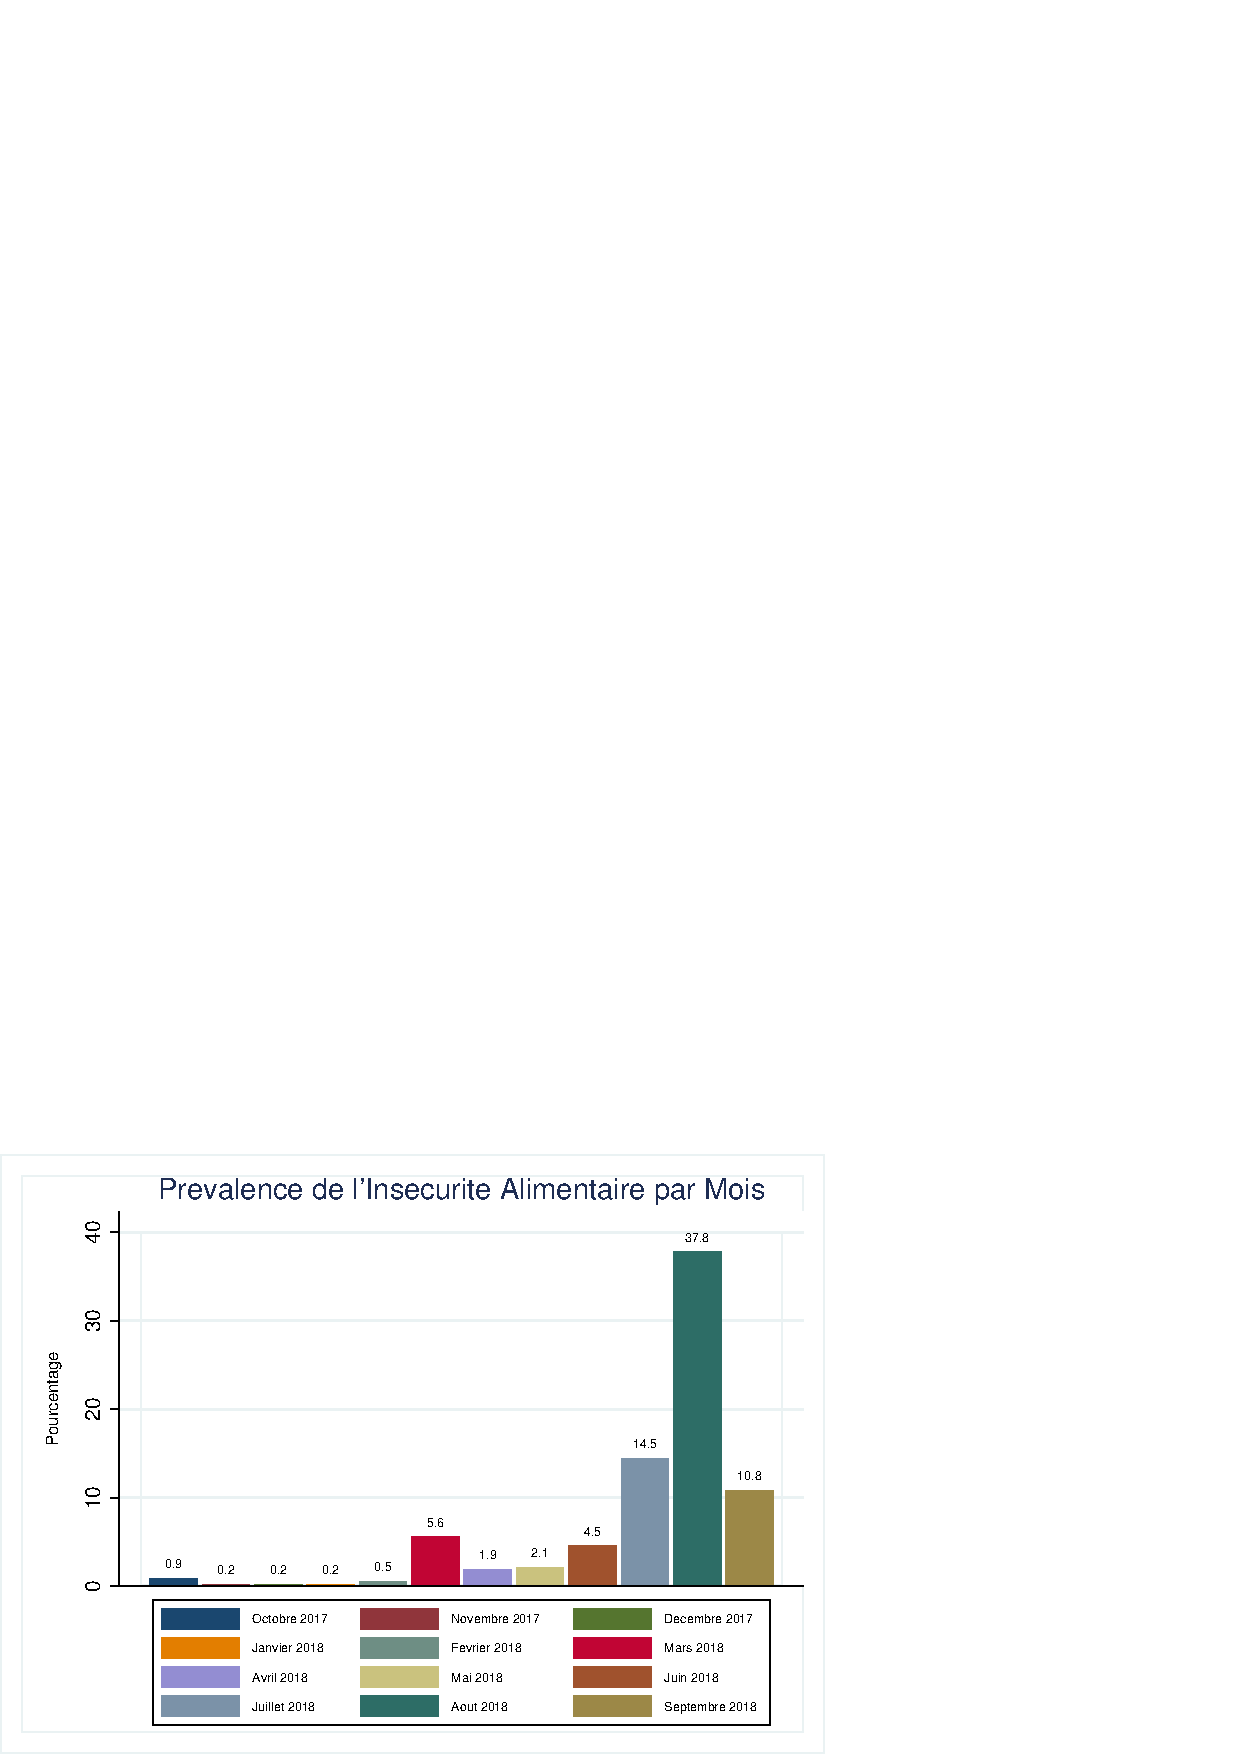
\includegraphics[width=0.9\linewidth]{FoodInsecure_bymonth.png}
\end{figure}
\FloatBarrier




\subsection{Research Design}
This study uses a Randomized Controlled Trial (RCT) to evaluate the impact of the Burkina Faso FIP PES, on participants' well being, measured by food security. We focus on the 2017 afforestation campaign running from August 2017 to May 2018. The figure ... shows the timeline for the different activities of this study in relation to the actual steps of the intervention. The 2017 reforestation campaign targeted about 33 sections of forest distributed across the 12 forests targeted by Burkina Faso FIP program. Each forest section includes two afforestation plots with about 400 newly planted trees. Right after the planting activities, the project team asked for volunteers to join a PES schemes, according to which they would receive a monetary payment based on the trees survival 9 months later. The project team's experience from previous years suggested that there would be oversubscription and that a selection would have to be made from the list of volunteers. In collaboration with the research team, the project team designed a public lottery strategy to decide on the participants to the program. The lottery-based participation assignment here is the fairest way to enroll people, and which would preserve he trust of the community members \citet{gueron2017politics}. The lotteries were conducted separately in each afforestation site \footnote{There is a total of 66 sites }, each yielding groups of 5 individuals who get to participate in this environmental cash transfer scheme - the \textit{treatment group} - and other individuals without access to the scheme - the \textit{control group}. Field agents representing the research team were present and helped the project teams implement smoothly these public lotteries. As we discuss in later sections of this paper, this lottery approach is the core of the identification strategy used for evaluating the impact of the intervention on participants' food security. \\

Immediately following the treatment assignment in the field, a survey team followed up with all those groups of 5 individuals who signed PES contracts, as well as 5 other randomly selected individuals amongst the non-selected groups, to collect baseline information on their socio economic characteristics and well being indicators.  These baseline information allowed us to check the validity of the randomization process. Table \ref*{tab:Balancing_tests}.. shows a balancing table comparing the treatment and the control groups. 


\begin{table}[ht!]
	\caption{Balancing table based on baseline characteristics}
	\centering
	\begin{adjustbox}{max width=1.0\linewidth}
	%	\begin{tabular}{@{\extracolsep{5pt}}lccccccc}
\\[-1.8ex]\hline \hline \\[-1.8ex]
  & \multicolumn{2}{c}{(1)}  & \multicolumn{2}{c}{(2)}  & \multicolumn{2}{c}{(3)} & \multicolumn{1}{c}{T-test}  \\
 & \multicolumn{2}{c}{PES}  & \multicolumn{2}{c}{non-PES}  & \multicolumn{2}{c}{Total}  & \multicolumn{1}{c}{Difference}  \\
  Variable & N & Mean/SE  & N & Mean/SE  & N & Mean/SE   & (1)-(2)  \\ \hline \\[-1.8ex] 
Age of respondent & 325 & \begin{tabular}[t]{@{}c@{}} 39.871 \\ (0.597) \end{tabular} & 305 & \begin{tabular}[t]{@{}c@{}} 38.433 \\ (0.621) \end{tabular} & 630 & \begin{tabular}[t]{@{}c@{}} 39.175 \\ (0.431) \end{tabular} &     1.438* \rule{0pt}{0pt}\\
Female respondent (1/0) & 325 & \begin{tabular}[t]{@{}c@{}} 0.123 \\ (0.018) \end{tabular} & 305 & \begin{tabular}[t]{@{}c@{}} 0.193 \\ (0.023) \end{tabular} & 630 & \begin{tabular}[t]{@{}c@{}} 0.157 \\ (0.015) \end{tabular} &    -0.070** \rule{0pt}{3ex}\\
Agriculture as primary activity (1/0) & 325 & \begin{tabular}[t]{@{}c@{}} 0.908 \\ (0.016) \end{tabular} & 305 & \begin{tabular}[t]{@{}c@{}} 0.885 \\ (0.018) \end{tabular} & 630 & \begin{tabular}[t]{@{}c@{}} 0.897 \\ (0.012) \end{tabular} &     0.022 \rule{0pt}{3ex}\\
Annual revenu from primary activity (LOG) & 325 & \begin{tabular}[t]{@{}c@{}} 3.057 \\ (0.411) \end{tabular} & 305 & \begin{tabular}[t]{@{}c@{}} 3.064 \\ (0.415) \end{tabular} & 630 & \begin{tabular}[t]{@{}c@{}} 3.061 \\ (0.292) \end{tabular} &    -0.007 \rule{0pt}{3ex}\\
Annual total revenu (LOG) & 325 & \begin{tabular}[t]{@{}c@{}} 9.893 \\ (0.526) \end{tabular} & 305 & \begin{tabular}[t]{@{}c@{}} 9.927 \\ (0.531) \end{tabular} & 630 & \begin{tabular}[t]{@{}c@{}} 9.909 \\ (0.374) \end{tabular} &    -0.035 \rule{0pt}{3ex}\\
Has a secondary activity (1/0) & 325 & \begin{tabular}[t]{@{}c@{}} 0.277 \\ (0.025) \end{tabular} & 305 & \begin{tabular}[t]{@{}c@{}} 0.262 \\ (0.025) \end{tabular} & 630 & \begin{tabular}[t]{@{}c@{}} 0.270 \\ (0.018) \end{tabular} &     0.015 \rule{0pt}{3ex}\\
Married (1/0) & 325 & \begin{tabular}[t]{@{}c@{}} 0.905 \\ (0.016) \end{tabular} & 305 & \begin{tabular}[t]{@{}c@{}} 0.862 \\ (0.020) \end{tabular} & 630 & \begin{tabular}[t]{@{}c@{}} 0.884 \\ (0.013) \end{tabular} &     0.042* \rule{0pt}{3ex}\\
Household size & 325 & \begin{tabular}[t]{@{}c@{}} 13.286 \\ (0.405) \end{tabular} & 305 & \begin{tabular}[t]{@{}c@{}} 12.666 \\ (0.467) \end{tabular} & 630 & \begin{tabular}[t]{@{}c@{}} 12.986 \\ (0.308) \end{tabular} &     0.621 \rule{0pt}{3ex}\\
Some formal schooling (1/0) & 325 & \begin{tabular}[t]{@{}c@{}} 0.182 \\ (0.021) \end{tabular} & 305 & \begin{tabular}[t]{@{}c@{}} 0.190 \\ (0.023) \end{tabular} & 630 & \begin{tabular}[t]{@{}c@{}} 0.186 \\ (0.016) \end{tabular} &    -0.009 \rule{0pt}{3ex}\\
Member of a forest management group (1/0) & 325 & \begin{tabular}[t]{@{}c@{}} 0.588 \\ (0.027) \end{tabular} & 305 & \begin{tabular}[t]{@{}c@{}} 0.538 \\ (0.029) \end{tabular} & 630 & \begin{tabular}[t]{@{}c@{}} 0.563 \\ (0.020) \end{tabular} &     0.050 \rule{0pt}{3ex}\\
Homestead far from the reforestation site (1/0) & 325 & \begin{tabular}[t]{@{}c@{}} 0.877 \\ (0.018) \end{tabular} & 305 & \begin{tabular}[t]{@{}c@{}} 0.944 \\ (0.013) \end{tabular} & 630 & \begin{tabular}[t]{@{}c@{}} 0.910 \\ (0.011) \end{tabular} &    -0.067*** \rule{0pt}{3ex}\\
Agric. Asset Index (PCA) & 325 & \begin{tabular}[t]{@{}c@{}} 0.132 \\ (0.093) \end{tabular} & 305 & \begin{tabular}[t]{@{}c@{}} -0.141 \\ (0.089) \end{tabular} & 630 & \begin{tabular}[t]{@{}c@{}} -0.000 \\ (0.065) \end{tabular} &     0.273** \rule{0pt}{3ex}\\
Household Asset Index (PCA) & 325 & \begin{tabular}[t]{@{}c@{}} 0.177 \\ (0.130) \end{tabular} & 305 & \begin{tabular}[t]{@{}c@{}} -0.189 \\ (0.068) \end{tabular} & 630 & \begin{tabular}[t]{@{}c@{}} 0.000 \\ (0.075) \end{tabular} &     0.366** \rule{0pt}{3ex}\\
Household landholdings (ha) & 265 & \begin{tabular}[t]{@{}c@{}} 15.668 \\ (4.077) \end{tabular} & 257 & \begin{tabular}[t]{@{}c@{}} 10.982 \\ (3.125) \end{tabular} & 522 & \begin{tabular}[t]{@{}c@{}} 13.361 \\ (2.579) \end{tabular} &     4.685 \rule{0pt}{3ex}\\
Land area cultivated (ha) & 265 & \begin{tabular}[t]{@{}c@{}} 4.923 \\ (0.233) \end{tabular} & 257 & \begin{tabular}[t]{@{}c@{}} 4.686 \\ (0.229) \end{tabular} & 522 & \begin{tabular}[t]{@{}c@{}} 4.806 \\ (0.163) \end{tabular} &     0.237 \rule{0pt}{3ex}\\
Total (nominal) food consumption expenditures in FCFA (past 7 days) & 325 & \begin{tabular}[t]{@{}c@{}} 11258.837 \\ (639.395) \end{tabular} & 305 & \begin{tabular}[t]{@{}c@{}} 11602.666 \\ (729.457) \end{tabular} & 630 & \begin{tabular}[t]{@{}c@{}} 11425.294 \\ (482.895) \end{tabular} &  -343.829 \rule{0pt}{3ex}\\
(LOG) Total (nominal) food consumption expenditures in FCFA (past 7 days) & 311 & \begin{tabular}[t]{@{}c@{}} 8.908 \\ (0.060) \end{tabular} & 300 & \begin{tabular}[t]{@{}c@{}} 8.875 \\ (0.068) \end{tabular} & 611 & \begin{tabular}[t]{@{}c@{}} 8.891 \\ (0.045) \end{tabular} &     0.033 \rule{0pt}{3ex}\\
Household Dietary Diversity Score (HDDS) & 325 & \begin{tabular}[t]{@{}c@{}} 4.425 \\ (0.080) \end{tabular} & 305 & \begin{tabular}[t]{@{}c@{}} 4.466 \\ (0.082) \end{tabular} & 630 & \begin{tabular}[t]{@{}c@{}} 4.444 \\ (0.057) \end{tabular} &    -0.041 \rule{0pt}{3ex}\\
\hline
\multicolumn{7}{@{} l}{F-test of joint significance (p-value)} &     0.121 \\
\multicolumn{7}{@{} l}{F-test, number of observations} &       517 \\
\hline \hline \\[-1.8ex]
%%% This is the note. If it does not have the correct margins, edit text below to fit to table size.
\multicolumn{8}{@{}p{2\textwidth}}
{\textit{Notes}:  The value displayed for t-tests are the differences in the means across the groups. The value displayed for F-tests are p-values. ***, **, and * indicate significance at the 1, 5, and 10 percent critical level. }
\end{tabular}

		\label{tab:Balancing_tests}
	\end{adjustbox}
\end{table}
\FloatBarrier

The table indicates that the treatment and control groups are fairly balanced ...


\newpage 
\section{Empirical Framework}

\subsection{Estimation Strategy}
We seek to estimate the average treatment effect of participation in the PES scheme on households' food security outcomes. This can be represented as:
\begin{equation}
\gamma = E[Y_{i1}-Y_{i0}]
\end{equation}

where $Y_{i1}$ and $Y_{i0}$, under the Rubin causal Model (RCM), represent the potential outcomes for individual i under alternative treatment status \citet{holland1986statistics,rubin1974estimating}. The core econometric strategy for the paper exploits the random assignment of individual members of the communities to a treatment group and a control group. The treatment group received and signed PES contracts with the project team, whereby they received monetary compensation based on the number of trees still alive, at verification, on the area assigned to them. The control group did not receive any contract, and hence no cash transfers from the project. Exploiting this exogenous treatment assignment, we estimate an intention-to-treat effect on household food security, using primarily the difference-in-means as estimator: 

\begin{equation} \label{eq:ATE_equation}
\widehat{\gamma} = \frac{1}{N{t}} \Sigma [Y_{i}|T_i=1] - \frac{1}{N{c}} E[Y_{i}|T_i=0]
\end{equation}

Under a completely randomized assignment of treatment, this estimator is unbiased for the average treatment effect. We base inference on the randomization distribution. This approach, still relatively uncommon in economics, has been strongly recommended for the analysis of randomized experiments such as ours \citet{athey2017econometrics,athey2017state,imbens2009recent}. To calculate the p-value associated with the estimated treatment effect, the randomized inference approach requires us to reassign the treatment status, keeping the number of treatment and control fixed, and calculate the corresponding difference in means. This process is repeated many times, and produces a distribution of treatment effect under the null hypothesis. The p-value we seek to calculate is simply the proportion of cases in which the fake treatment effect estimated is at least as large in absolute value to the estimate we seek to test. The method is attractive because it is non parametric and relies less on modelling assumptions encountered in regression frameworks.  \\ 

Nevertheless, we also adopt the commonly used regression framework, as alternative approach. Although not originally meant for the analysis of data from randomized experiments, regression analyses use parametric modelling and allow us to use covariates adjustments to improve the precision of our estimates, remove biases when the randomization was not adequate, and make the analysis more informative. In particular given that the stratified nature of our randomization process performed separately within each forest bloc, the regression analysis allows us to control for forest bloc dummies and improve treatment effects precisions. The core regression specification takes the following form: 

\begin{equation} \label{eq:linear_reg_model}
Y_{i}=\alpha +\beta x_{i}  + \gamma T_i +\mu_{i}
\end{equation}

where $Y_{i}$ is a measure of food (in)security experienced by household $i$, $x_{i}$ is a vector of control variables, $T_i$ is the treatment assignment variable taking values 1 if a household was offered the opportunity to participate in the PES scheme, and zero otherwise. In this equation, $\gamma$ is the main parameter of interest. $\mu_{i}$ is an unobserved error term assumed to be random. We estimate $\gamma$ by applying Ordinary Least Squares (OLS) to Equation \ref{eq:linear_reg_model} above, an estimator which essentially minimizes the sum of squared residuals.  \\

%\subsection{Identification Strategy}

Dealing with Spillover \\

Dealing with multiple hypotheses testing biases \\


Our outcomes of interest include both discrete and continuous classes of indicators capturing the food security status of the household. \\


\newpage 
\section{Data and Descriptive Statistics}

\subsection{Data Sources}

During the tree planting, 660 individuals, equally distributed into treatment and control groups, were enrolled into this study. Right after the PES contracts were signed with farmers, a baseline survey was rolled out between September-October 2017 [DOUBLE CHECK SURVEY DATE], tracking the original sample down to their households in their villages. The survey team found 630 out of the 660 individuals included in the study: 305 control households, and 325 treatment households.  The survey instrument included modules capturing households' demographic characteristics, asset ownership, and food consumption. Using a balancing table [SEE APPENDIX], we compare these two groups of individuals to validate the randomization process. \par

A follow up survey was undertaken, around September-October 2018, approximately 3 months after the monetary transfers were distributed to participants based on trees survival. This follow up survey uses a similar instrument as the baseline, except with an extension of the food security module. During this phase, the survey team was able to find 574 out of 630 households interviewed at baseline, implying a relatively low attrition rate of about 9 percent, fairly balanced across treatment and control households\footnote{The difference in attrition rate between treatment and control groups was faily low (0.044 percentage points), and was significant only at 10 percent}. We therefore do not fear any bias resulting from attrition.  Nevertheless, we re-conduct balancing tests on the non-attrited sample to confirm balancedness between treatment and control groups [INCLUDE THIS TABLE IN APPENDIX].


\begin{table}[ht!]
	\caption{Attrition Rate by Treatment}
	\centering
\begin{adjustbox}{max width=1.0\linewidth}
\begin{tabular}{@{\extracolsep{5pt}}lccccccc}
\\[-1.8ex]\hline \hline \\[-1.8ex]
  & \multicolumn{2}{c}{(1)}  & \multicolumn{2}{c}{(2)}  & \multicolumn{2}{c}{(3)} & \multicolumn{1}{c}{T-test}  \\
 & \multicolumn{2}{c}{controle}  & \multicolumn{2}{c}{traitement}  & \multicolumn{2}{c}{Total}  & \multicolumn{1}{c}{Difference}  \\
  Variable & N & Mean/SE  & N & Mean/SE  & N & Mean/SE   & (1)-(2)  \\ \hline \\[-1.8ex] 
Participant trouvé (Oui=1, Non=0) & 305 & \begin{tabular}[t]{@{}c@{}} 0.889 \\ (0.018) \end{tabular} & 325 & \begin{tabular}[t]{@{}c@{}} 0.932 \\ (0.014) \end{tabular} & 630 & \begin{tabular}[t]{@{}c@{}} 0.911 \\ (0.011) \end{tabular} &    -0.044* \rule{0pt}{0pt}\\
\hline \hline \\[-1.8ex]
%%% This is the note. If it does not have the correct margins, edit text below to fit to table size.
\multicolumn{8}{@{}p{1\textwidth}}
{\textit{Notes}:  The value displayed for t-tests are the differences in the means across the groups. ***, **, and * indicate significance at the 1, 5, and 10 percent critical level. }
\end{tabular}

		\label{tab:Attrition_byTraitement}
\end{adjustbox}
\end{table}
\FloatBarrier


\subsection{Food Security Measures}
The definition of food security proposed since the 1996 World Food Summit has been widely agreed upon, by practitioners and researcher alike.\footnote{It states that: "Food security exists when all people, at all times, have physical and economic access to sufficient, safe and nutritious food to meet their dietary needs and food preferences for an active and healthy life".} However, there is a significant variety of indicators used to measure food security, all of which have drawn some form of criticism. This is due to the difficulty of finding a single indicator that captures satisfactorily all dimensions of food security implied by the formal definition (availability, access, utilization, stability). While there has been recent advocates for harmonizing food security measures \cite{carletto2013towards} [ALSO CITE BARRET], multiple indicators remain available for researchers and practitioners to chose from.   
Our enline survey instrument included an extended food security module, which allows us to generate the following commonly used food security measures at the household level and explore treatment effects of the BF FIP PES Scheme.  \par

\begin{itemize}
	
	\item The Household Food Consumption Expenditures 
	Definition, computation, weakness, citation, descriptives

	\item The Household Dietary Diversity Score 

	\item The Household Hunger Scale	
	
	\item The Household Food Insecurity Access Scale  
	Another way of capturing household food insecurity status is the Household Food Insecurity Access Scale (HFIAS). This indicator captures ... It creates 4 categories of food security depending on the severity of food insecurity. Figure \ref{fig:HFIAS} shows the distribution of our sample households into the 4 categories of food insecurity. Overall, 33 percent of the group suffers some form of food insecurity, and are distributed almost equally across the midly food insecure, the moderately food insecure, and the severely food insecure categories. \\
	
	
	\begin{figure}[ht!]
		\footnotesize
		\centering
		\caption{PES and Food Security: OLS Results \label{fig:HFIAS}}
		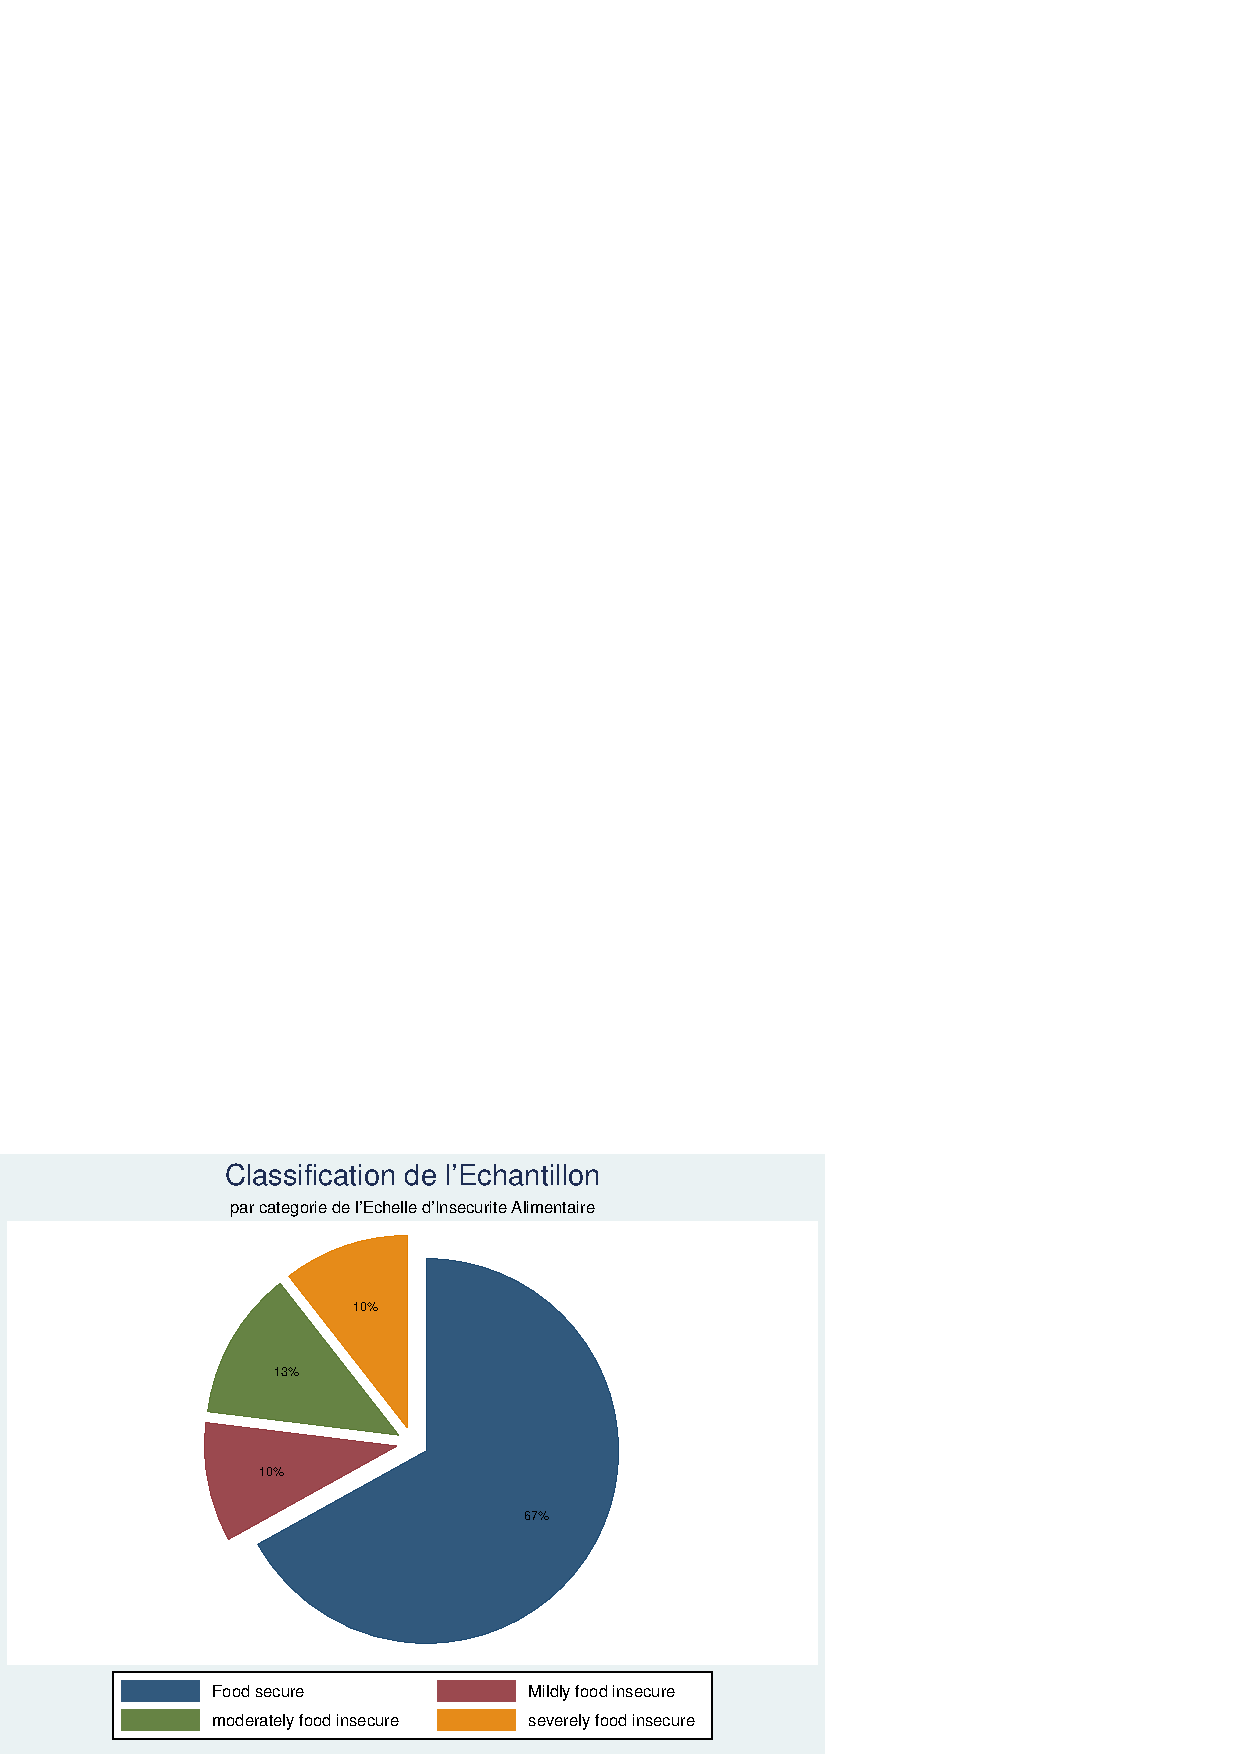
\includegraphics[width=0.9\linewidth]{Food_Insecure_HFIApie.png}
	\end{figure}
	\FloatBarrier
	

		
\end{itemize}







\newpage
\section{Results and Discussion}

We begin this section by presenting non-parametric evidence of the relationship between participation in the above described PES scheme and food security outcomes. Given exogenous variation in treatment assignement, these non-parametric estimates are unbiased for the intention to treat effects of interest, and not expected to be influenced by confounding factors.  \\



Nevertheless we follow this presenting the parametric results as described in our empirical framework section, accounting from other household characteritics, in order to improve the prcision of our estimates.  \\

We finally explore evidence of treatment heterogeneity by testing if the observed effects hold   



%\begin{table}[ht!]
%	\caption{Food Security Indicators by Treatment}
%	\centering
	%\begin{adjustbox}{max width=1.0\linewidth}
		\begin{tabular}{lcccccc} \hline \hline
                  &                      & (1)         &                               & (2)           &         & Randomization \\            
                  &                      & PES     &                           & non-PES   & t-test  & inference         \\            
 Variable & N/[Clusters] & Mean/SE &  N/[Clusters] & Mean/SE   & p-value & p-value       \\ \hline 
                                   Total (nominal) food consumption expenditures in FCFA (past 7 days) & 303 & 12940.488 & 271 & 11097.077 & 0.041 & 0.041 \\    &  & (690.208) &  & (655.157) &  &  \\  (LOG) Total (nominal) food consumption expenditures in FCFA (past 7 days) & 303 & 9.147 & 271 & 9.022 & 0.033 & 0.035 \\   &  & (0.047) &  & (0.046) &  &  \\  Household Food Insecurity Access Scale (HFIAS) \in [0,4] & 303 & 0.931 & 271 & 1.517 & 0.000 & 0.000 \\   &  & (0.108) &  & (0.132) &  &  \\  HFIAS = 1 (food secure) & 303 & 0.736 & 271 & 0.594 & 0.000 & 0.000 \\   &  & (0.025) &  & (0.030) &  &  \\  HFIAS = 4 (severely insecure) & 303 & 0.063 & 271 & 0.151 & 0.000 & 0.000 \\   &  & (0.014) &  & (0.022) &  &  \\  Household Hunger Scale (HHS) \in [0,3] & 303 & 0.155 & 271 & 0.336 & 0.000 & 0.000 \\   &  & (0.030) &  & (0.044) &  &  \\  HHS = 1 (no hunger) & 303 & 0.964 & 271 & 0.882 & 0.000 & 0.000 \\   &  & (0.011) &  & (0.020) &  &  \\  HHS = 2 (moderate hunger) & 303 & 0.036 & 271 & 0.118 & 0.000 & 0.000 \\   &  & (0.011) &  & (0.020) &  &  \\  Household Dietary Diversity Score (HDDS) & 303 & 3.878 & 271 & 3.845 & 0.781 & 0.790 \\   &  & (0.082) &  & (0.085) &  &  \\       \hline
\multicolumn{7}{@{}p{1.2\textwidth}}
{\textit{Notes}: We show both standard p-values and p-values computed by randomization inference (RI) with 1000 repetitions.}
\end{tabular}

%		\label{tab:Food_Consumption_Indices}
	%\end{adjustbox}
%\end{table}
\FloatBarrier


\subsection{PES and Food Consumption Expenditures}

According to Engel law, the poor spend a relatively high proportion of additional income on food. This suggests that, the Burkina Faso PIF PES participants will likely allocate a greater share of the environmental cash transfers they receive to food consumption, thereby improving  food security outcomes for their households.

 Figure ... presents the Kernel density estimates of the distribution, in logarithm form, of the reported household food consumption expenditures during the 7 days prior to the survey date for participants and non-participants in the PES scheme. Consistent with the above hypothesis, the weekly food consumption expenditures for the PES participants is distributed to the right of the distribution for the non participant. In table \ref*{tab:Food_Consumption_Indices}, we show mean difference for each food security indicator, as well as the t-test inference results of significance of such difference. The table shows that the mean food consumption expenditure is about 12940 FCFA for the participants, and about 11097 FCFA for the non participants. This suggests a positive intention to treat effect of 1843 FCFA corresponding to a 12.5 percent increase in weekly food consumption expenditure. The p-value based on the randomized inference is ... (See figure ...) suggesting our estimated intention to treat effect is significant at 10 percent. This is also consistent with the p-value from the t-test.   \par

\begin{figure}[ht!]
	\footnotesize
	\centering
	\caption{Distribution of Household Food Consumption Expenditures by Treatment \label{fig:map_overview}}
	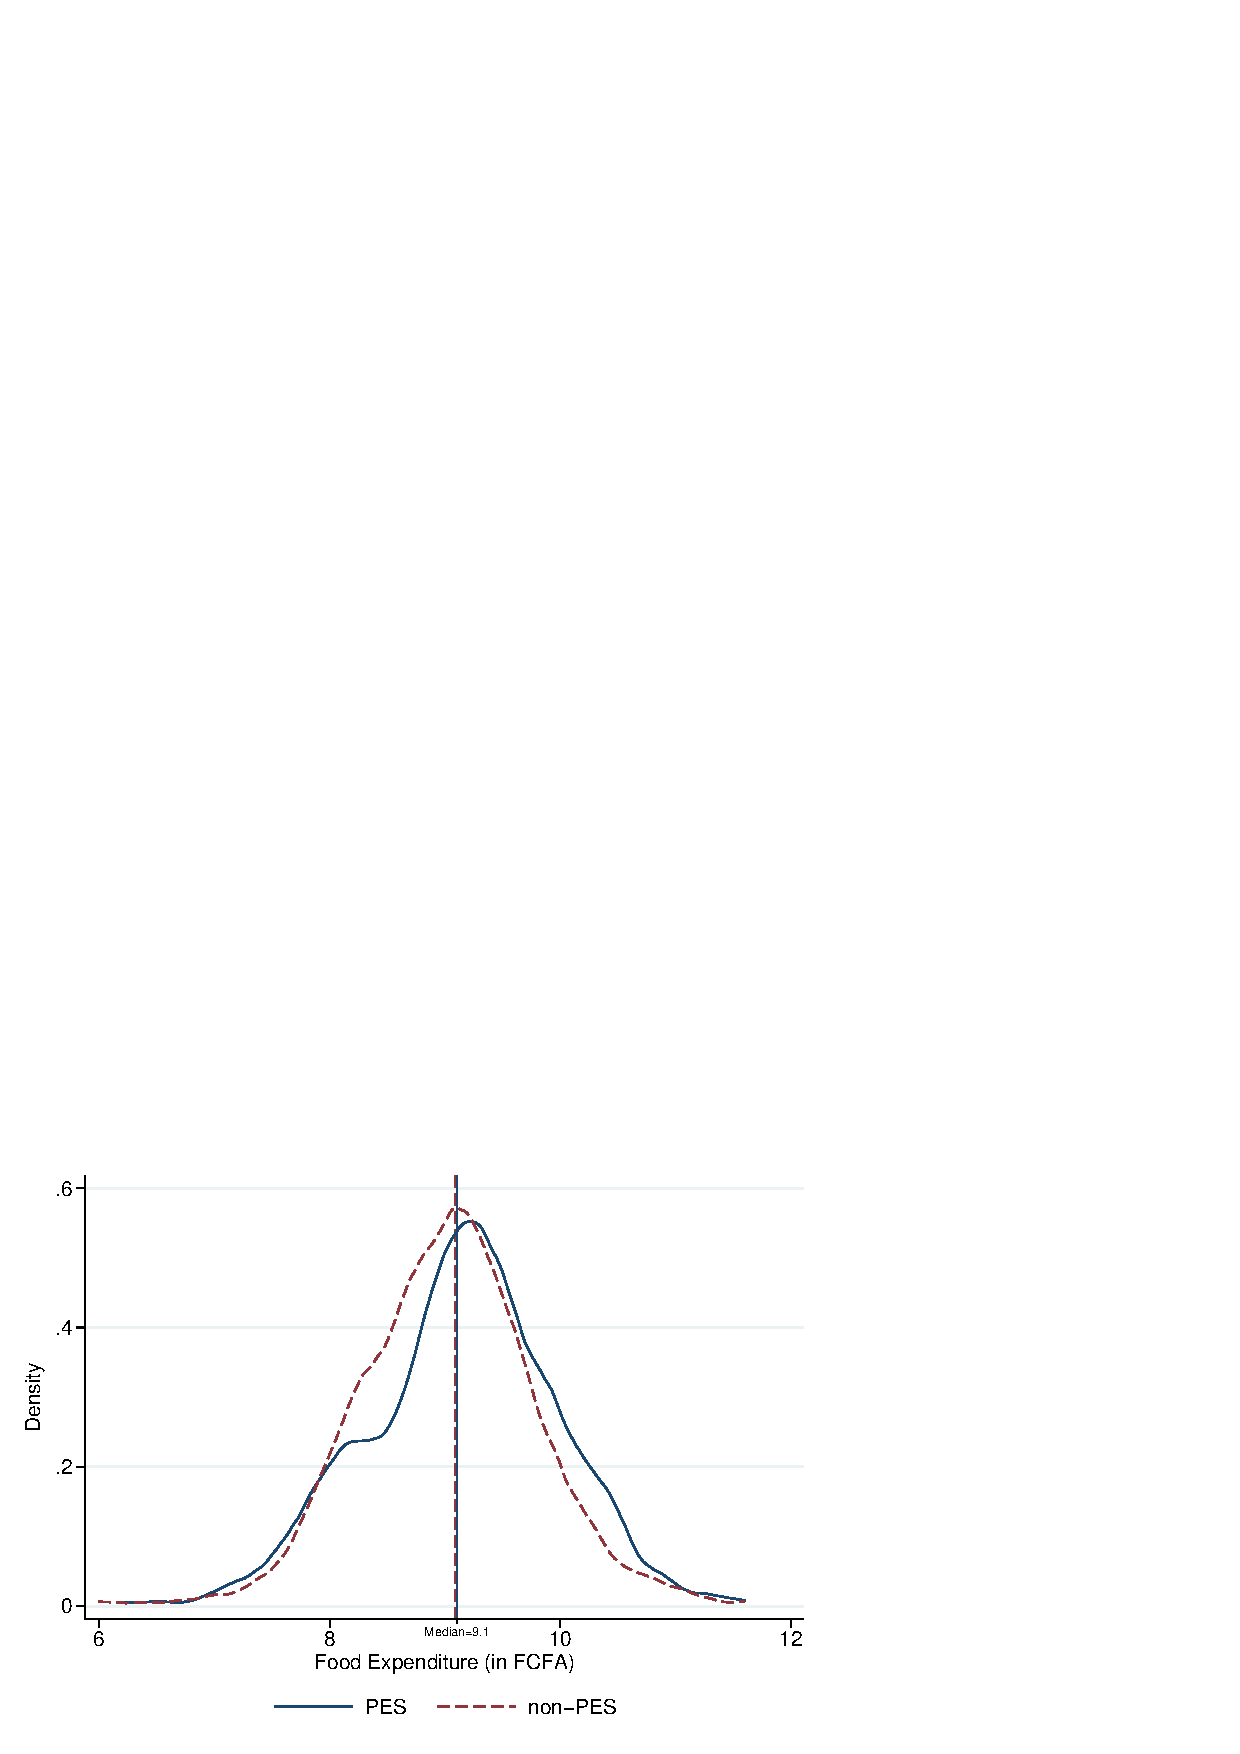
\includegraphics[width=0.9\linewidth]{kdensity_LOG_FoodConsExp.png}
\end{figure}
\FloatBarrier



The data used for this study includes dissagregated expenditures in different food groups. We explore, which food groups benefited particularly from the increased food consumption expenditure as a results of the environmental cash transfer. Figure \ref{fig:food_exp_bygroup} is a bar graph stacking up the food consumption expenditures in each food group, to make up the total food consumption expenditure value, seperatly for the participants and non participants in the PES scheme. The graph suggests that the largest part of the increase in food consumption expenditure as a result of the cash transfer, went to cereals, roots and tubers, which were already taking up more than 50 percent of the household food expenditure. This implies that although there is a positve and significant effect of these environmental cas tranfer on nominal food consumption expenditures, they did not translate into improved dietary diversity for the household. As a confirmation, we compare the distribution of household dietary diversity score between participants and non participants (see Figure \ref{fig:HDDS}), and found no significant difference. The p-value for the Smirnov Kolmogorov test of equality of the two distribution returns a value of 0.99 suggesting no evidence of statistical difference between the two distributions.


\begin{figure}[t]
	\footnotesize
	\centering
	\caption{Average Food Expenditure Shares by Food Groups  \label{fig:food_exp_shares}}
	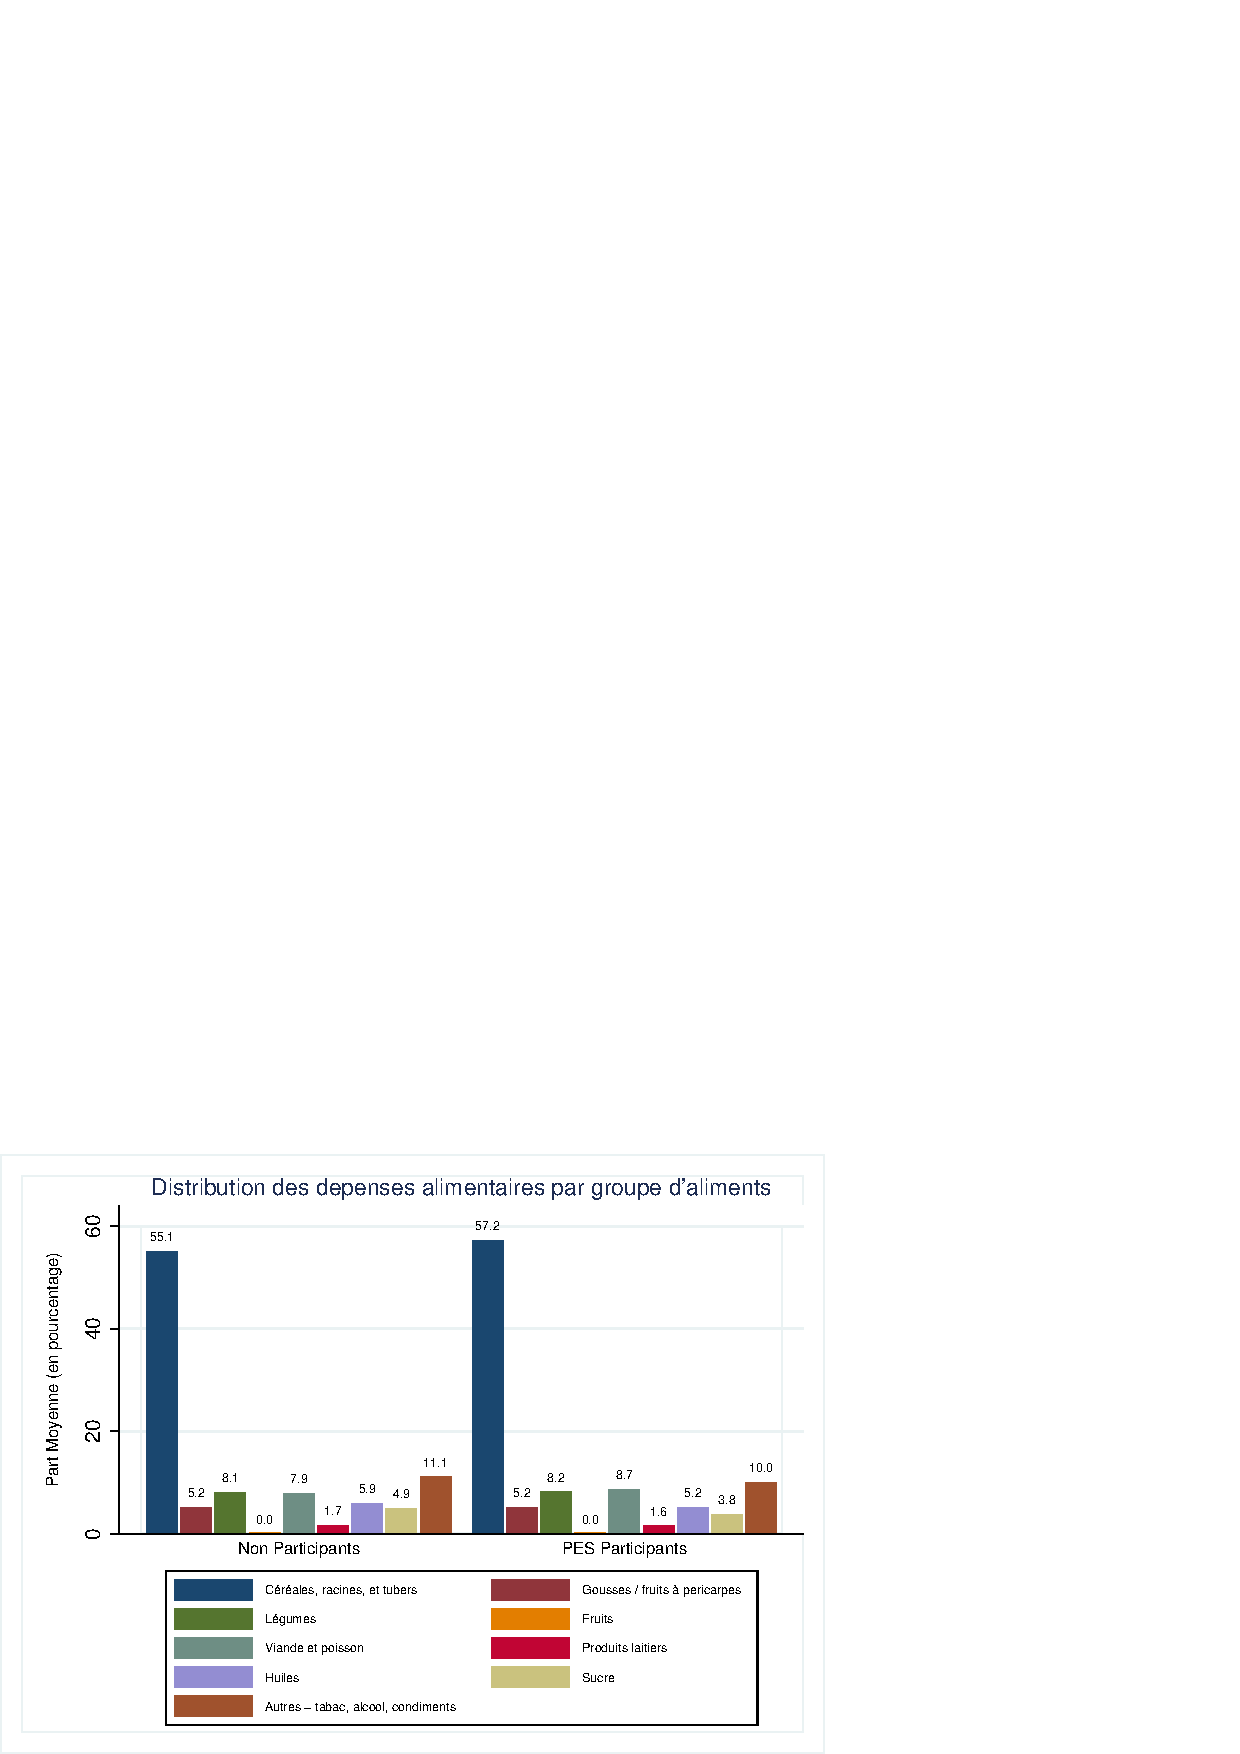
\includegraphics[width=0.9\linewidth]{FoodConsExpShr_byfoodgroup.png}
\end{figure}
\FloatBarrier



\begin{figure}[ht!]
	\footnotesize
	\centering
	\caption{Average Food Expenditure by Food Groups  \label{fig:food_exp_bygroup}}
	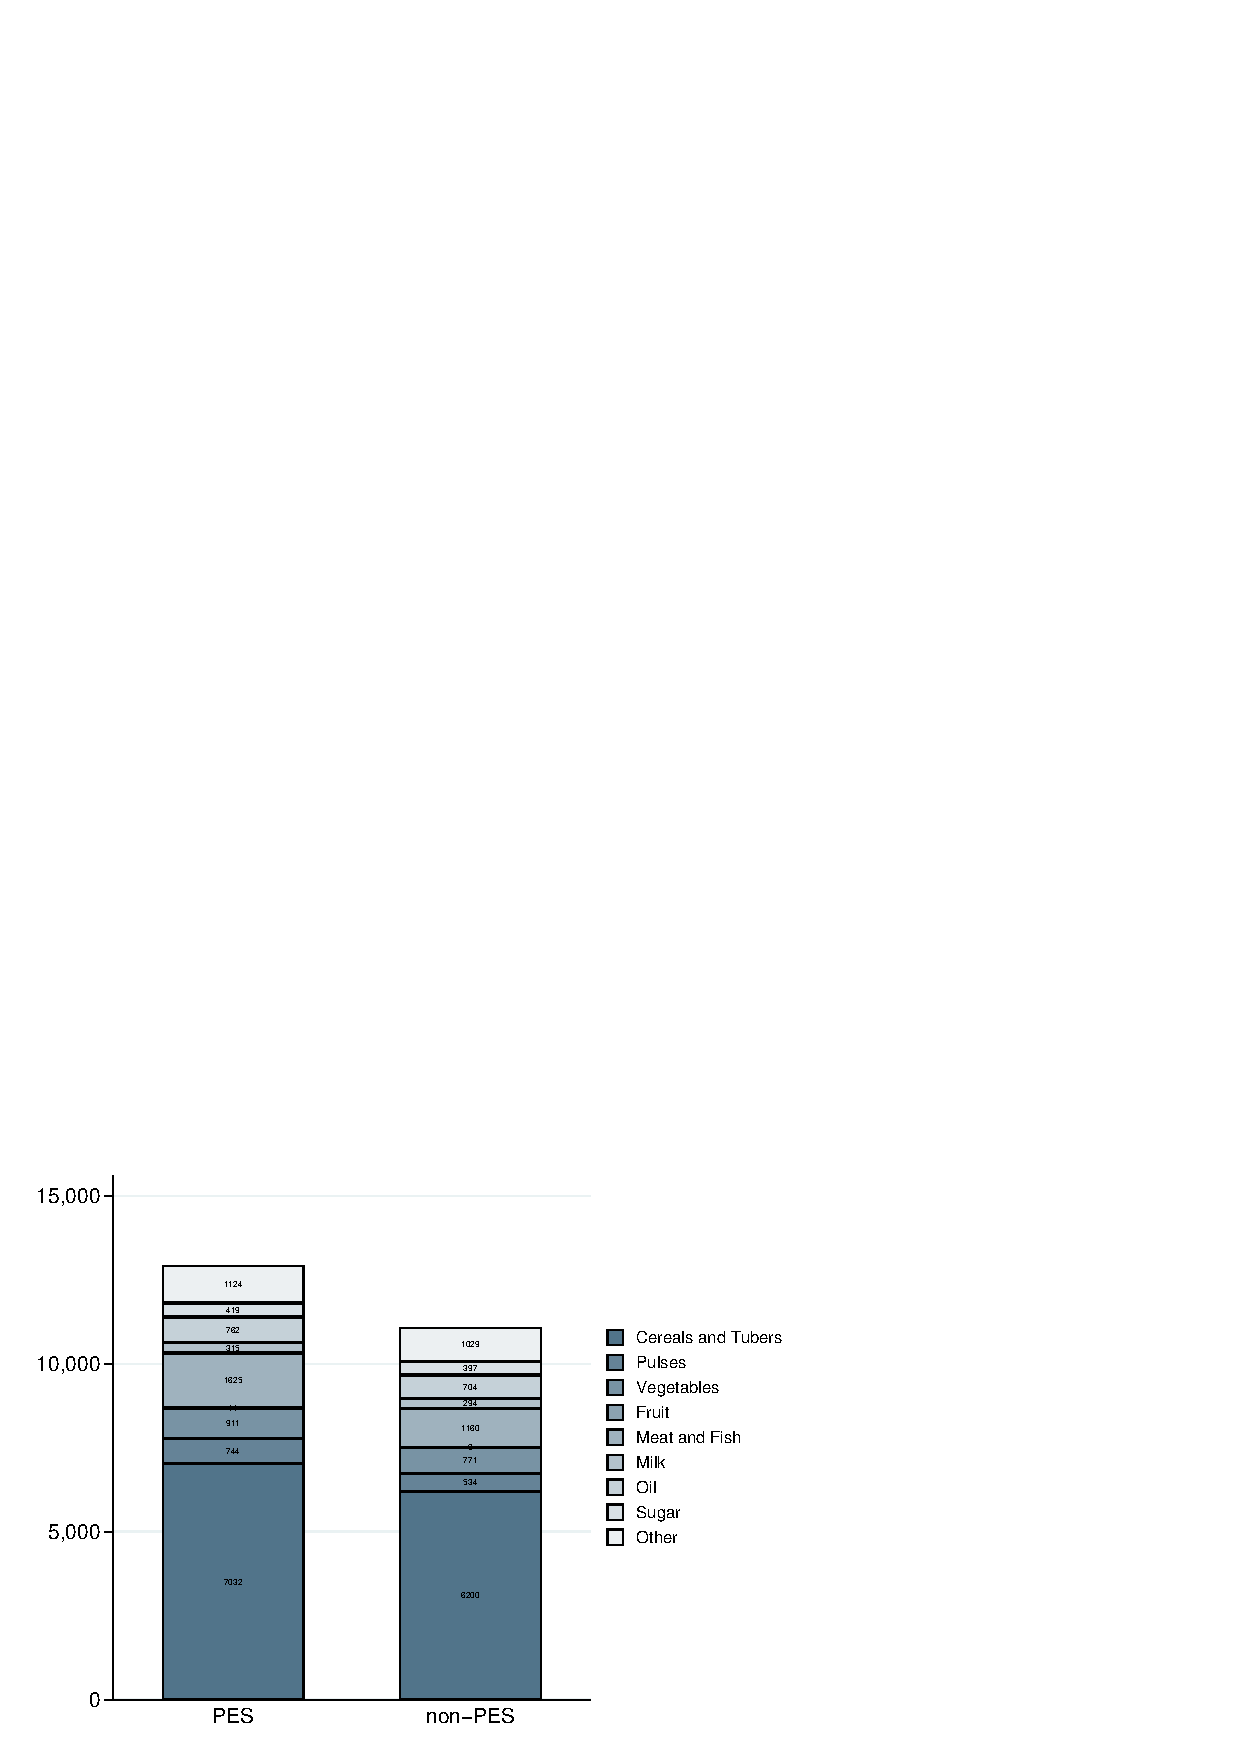
\includegraphics[width=0.9\linewidth]{FoodConsExp_byfoodgroup_stack.png}
\end{figure}
\FloatBarrier


\begin{figure}[ht!]
	\footnotesize
	\centering
	\caption{Distribution of Household Dietary Diversity Score by Treatment  \label{fig:HDDS}}
	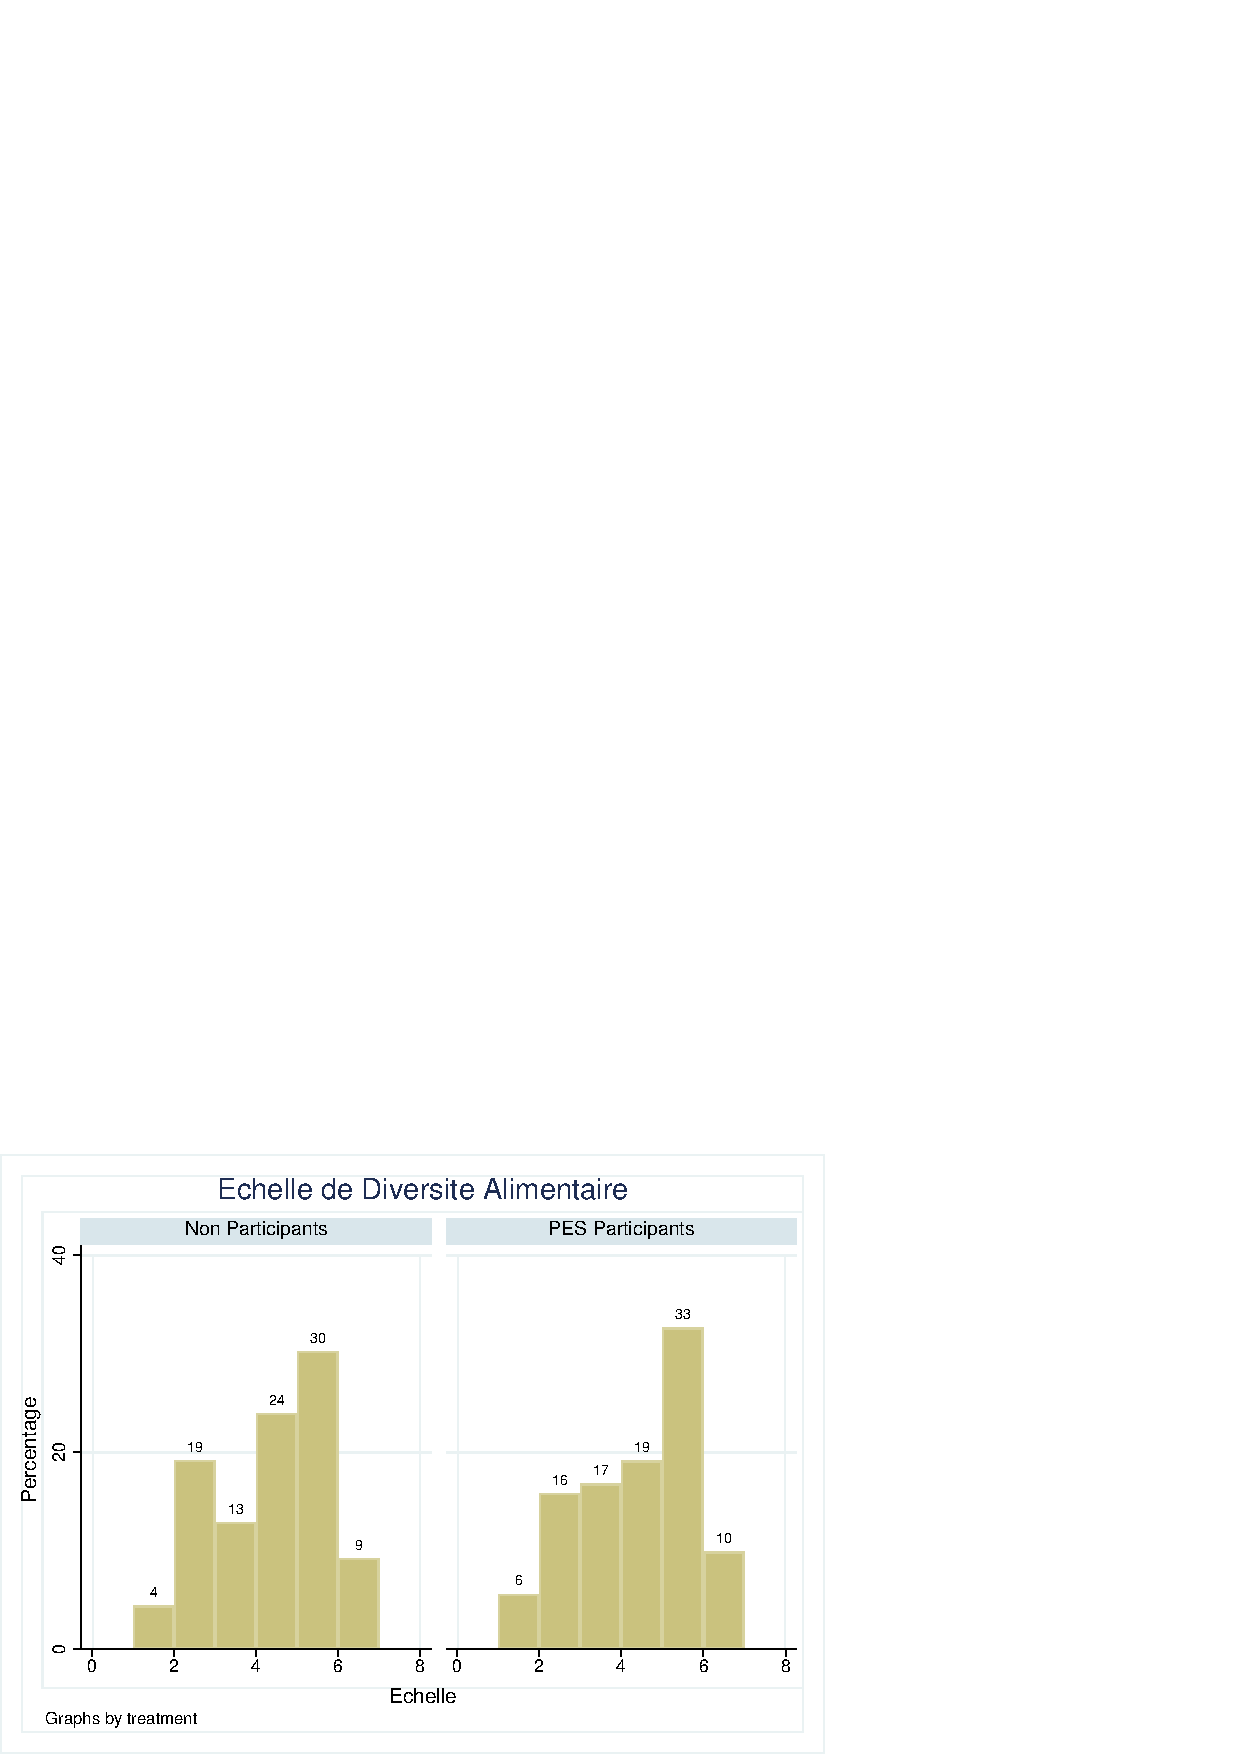
\includegraphics[width=0.9\linewidth]{DiversiteAlimentaire.png}
\end{figure}
\FloatBarrier

\clearpage
\subsection{PES and Household Food Insecurity Experience Scale and Hunger Scale}

Comparing the treatment and control groups, Table \ref*{tab:Food_Consumption_Indices} shows that the raw HFIAS score is lower in the treatment group compared to the control group. The difference in HFIAS between the two groups is 0.586, statistically significant at 1 percent. This results is confirmed when we compare the treatment and the control groups in terms of the proportion of people who experienced some form of food insecurity, or in terms of the probability fo experiencing severe food insecurity. Table \ref*{tab:Food_Consumption_Indices} shows an estimate of food insecurity prevalence of about 14.2 percentage points more amongst treatment individuals compared to control ones, statistically significant at 1\%. With an average of ... amongst the control group, this difference correspond to almost 25 percent reduction in the prevalence of food insecurity. The results are even stronger when we look at the prevalence of severe food insecurity. The percentage of people falling in the severe food insecurity category is about 6\% in the treatment group, compared to 15\% in the control group, suggesting more than 50\% reduction. These results are better illustrated on the Figure \ref*{fig:HFIAS_impact} below.  \\

\begin{figure}[ht!]
	\footnotesize
	\centering
	\caption{PES and Food Security: OLS Results \label{fig:HFIAS_impact}}
	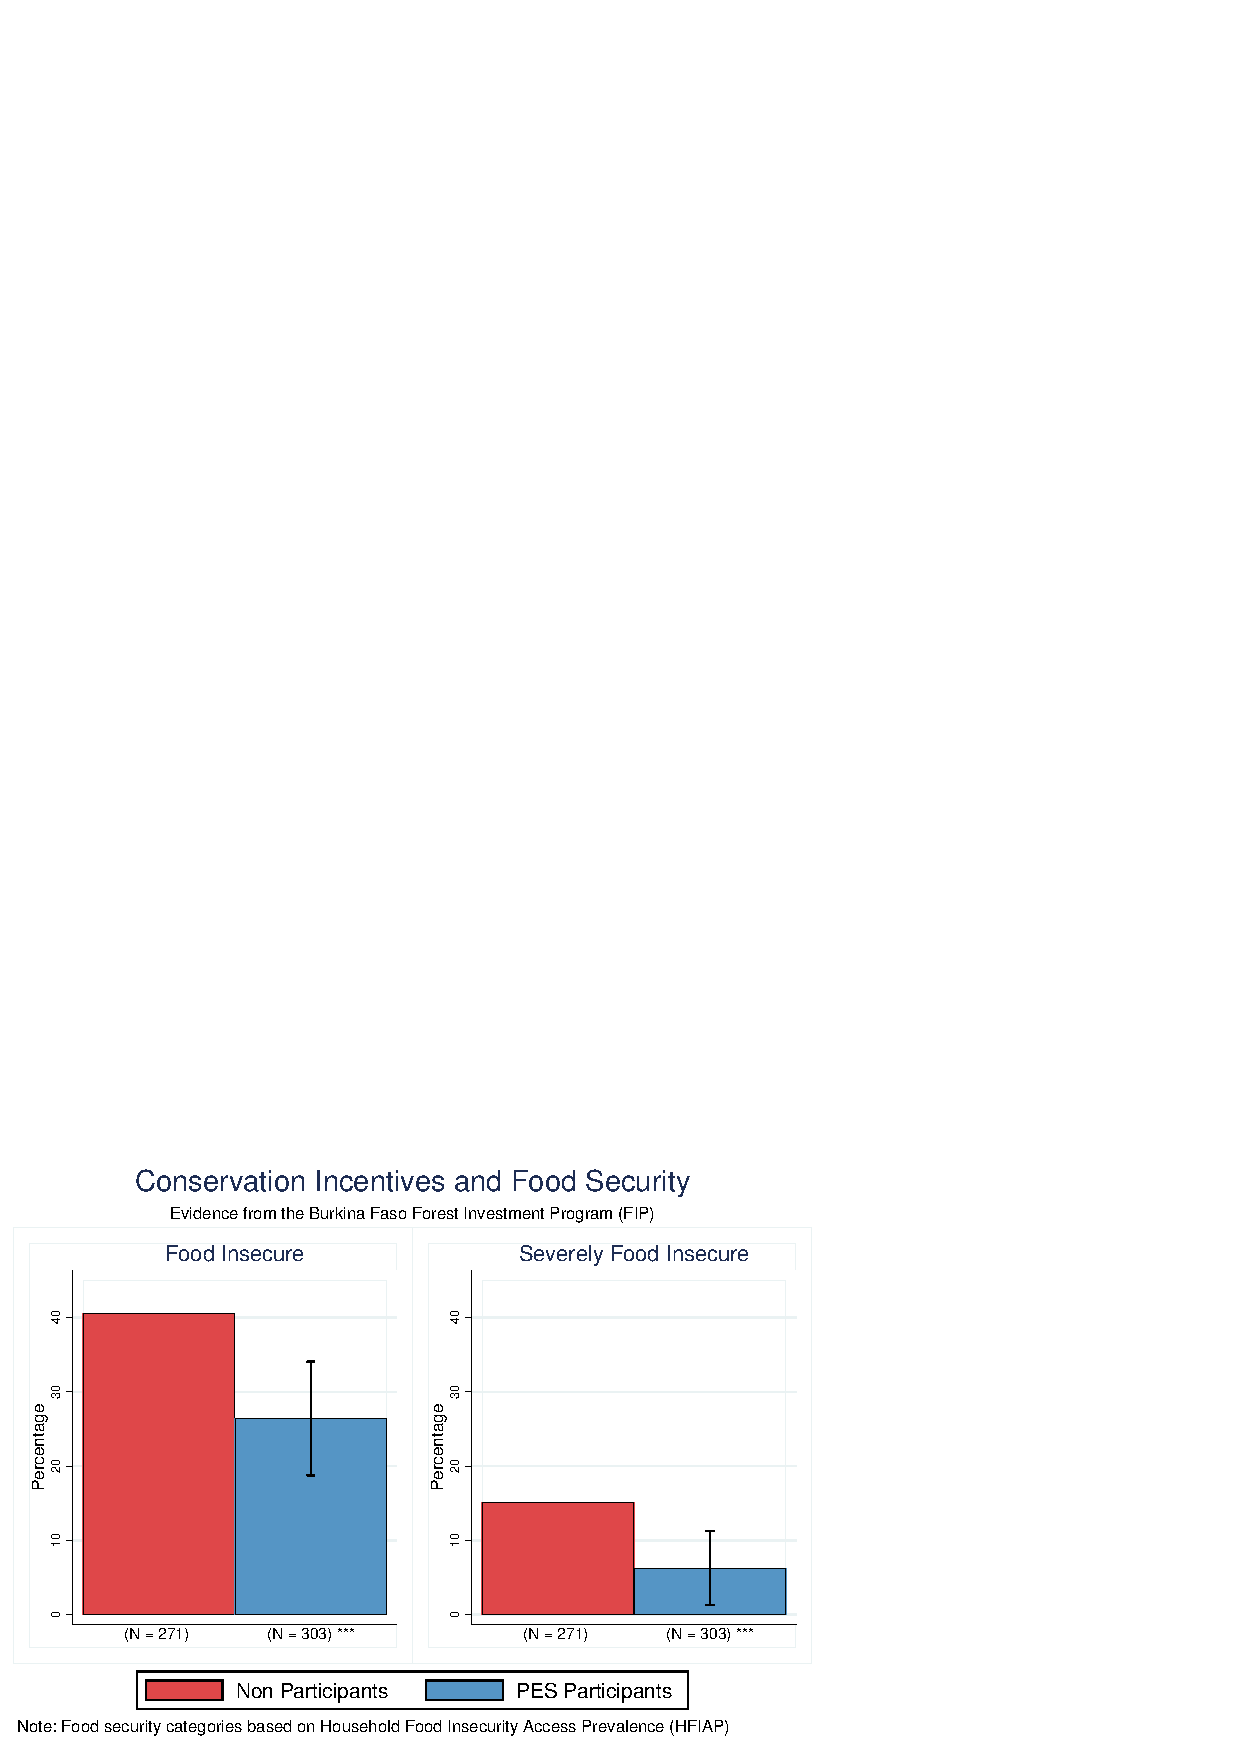
\includegraphics[width=0.9\linewidth]{Food_Insecure_graph.png}
\end{figure}
\FloatBarrier

The results on the HFIAS are almost exactly replicated when we consider the Household Hunger Scale as food security indicator. As shown in Table \ref*{tab:Food_Consumption_Indices}, the participation in the environmental cash transfer scheme seems to have reduced by almost 70\% the proportion of household who experienced hunger during the month prior to the survey. 

All of these suggest a positive relationship between participation in PES and food security status. Given the random assignment of treatment status, these non parametric estimates can be interpreted as causal. Nevertheless we turn to parametric estimation approaches to ... adress heterogenity of treatment effects and potential spillover issues... \\


\newpage
\subsection{Regression estimates - heterogeneous impacts}
 
Table .. summarizes the OLS estimation results of Equation \ref{eq:linear_reg_model}, ...

The regression results are consistent with the difference in mean estimates, with smaller variances.


\newpage
\subsection{Robustness Checks}


%\begin{table}[ht!]
%	\caption{NDVI Regression results - Panel data FE}
%	\centering
%	\begin{adjustbox}{max width=1.0\linewidth}
%		\input{ndvi_FE_Results.tex}
%		\label{tab:NDVI FE regression results}
%	\end{adjustbox}
%\end{table}



\clearpage
\newpage
\section{Conclusion}

We have used data on 630 households across 32 communes in Burkina Faso, to investigate the causal relationship between participation in PES schemes and 
houehold welfare, by examining whether participation in a government-led conservation incentive schemes has protected houshold against food insecurity during the pre harvest-period.  \\

Our results show that ... participation in PES increase the likelihood of a household been food insecure by 14 percentage points on average, and the likelihood that a housholds falls into the severely food insecure category by 9 percentage points.  \\

These are important results because ... first experimental evidence of the impacts of PES on houshold welfare. \\

From a policy perspective, our findings suggests that there is potential for creating further synergies between environmental and social protection goals, given that the primary agents for climate change mitigation actions are also the same agents who need help the most in coping with extreme poverty worsened by the negative effects of climate shocks and variations. Beyond food security, other dimensions of household welfare, such as youth employment, gender inclusion, and rural entrepreneurship, can be built explicitely into environmental projects to achieve maximum impacts from each dollars invested in development interventions.    \\

As in any empirical work, the study contains a number of limitations worth emphasizing. First [internal validity] ... We could not fix this using the data at hand ... ???
Second [external validity] ... Finally ...
Future research with experimental design on the topic will help us gather enough evidence across contexts, also accross a set of outcomes, to establish whether this causal relationship we identify in this study, is an empirical regularity.






\clearpage
\newpage
\section*{References}
\bibliography{mybibfile}

\end{document}